\chapter{Lab 10\&11}
\setcounter{TASignatures}{0}
\setcounter{AsideCounter}{0}

\section{Introduction}
    \vspace{0.1em}

    \textbf{In this lab you gain experience with:}
    \begin{enumerate}
        \item Programming State Machines in Ladder Logic
    \end{enumerate}

\subsection{Lab Files}

Go to iLearn and download the PLC and HMI files for this lab to the PC. Then download the PLC project to the PLC and the HMI application to the HMI. 

\subsection{Acceptable Instructions}

You may have previous experience with PLCs and that is great! However, you are only allowed to use the instructions that we have covered thus far in the lab. So, if you have experience already, consider it a challenge to restrict yourself to only use the instructions that have been covered thus far in lecture to solve the problem!

\subsection{Lab agreement}

The planning of a program is often a very social activity, however the actual writing of the code is always an individual pursuit. In this class it is very much the same. Students are welcome to verbally assist each other, but each person is required to write their own code and personally complete each lab. In this way each student will gain valuable experience with programming PLCs. 

\textbf{The undersigned person guarantees that any and all work demonstrated to the TA in regard to this lab is a result of their own work with no unauthorized help.}

\signatureSlot{Student}


\section{Simple State Machine}
Notice that there is no associated object for this lab. You must create all the necessary tags and HMI objects to fulfill the requirements outlined in this exercise. Make sure that the HMI page you make looks \textit{very} professional. 

This lab deals with state machines. In general you will need to fully define any state machine which you intend to program. However, in this part of the lab you are given the plain English description and the enumeration of states, inputs, and outputs.
\\

After successfully providing the pneumatic road tube machine to Wamapoke County, you were contacted again to do some additional work for Pawnee. They are adding a traffic light near town hall and would like you to program the light using an Allen Bradley PLC. 

As a constraint, they require any stoplight installations in Wamapoke county be programmed using state machines. They had an installation programmed by a fellow named Nadha Scolar that did not work well. It was observed that he did not use state machines. Therefore, state machines are now a required standard for all new Wamapoke stoplight controllers.

You may have never considered using state machines in a PLC before, so you are going back to your lair and develop a proof of concept as to how a state machine should work in a PLC.




\subsection{Plain English Description}

You are to program a state machine that will demonstrate how state machines work (similar to the one demonstrated in lecture with a few differences). The state machine is to have 3 states. They are to be called \verb|State1|, \verb|State2|, and \verb|State3|. \verb|State1| should be programmed to be the default state.

There are three inputs: \verb|transition1|, \verb|transition2|, and \verb|transition3|. The inputs are to be connected to buttons on the HMI. You are to draw the state machine diagram on the HMI and use it to show the current state. The transition buttons should be shown over top of the transition lines between the states. 

The outputs will be \verb|Show_State1|, \verb|Show_State2|, and \verb|Show_State3|. You are to use these outputs to show the current state on the state machine diagram on the HMI. Do not simply display the current state number. You are to display the current state in the same way demonstrated in the lecture practical. (This is to help you to continue getting better at HMI development.)

When the machine is in \verb|State1| and \verb|transition1| occurs, the machine should transition to \verb|State2|. When the machine is in \verb|State2| and \verb|transition2| occurs, the machine should transition to \verb|State3|. When the machine is in \verb|State3| and \verb|transition3| occurs, the machine should transition to \verb|State1|. 

\aside{In the practical example in the lecture for state machines, it was necessary to detect the rising edge of the change state button. This will \textit{not} be necessary here as each state has unique signals associated with the state transition.}


\TASignatureSlot



\section{Challenge - Toggle... Again}
Notice that there is no associated object for this lab. You must create all the necessary tags and HMI objects to fulfill the requirements outlined in this exercise. Make sure that the HMI page you make looks \textit{very} professional. 

This lab deals with state machines. In general you will need to fully define any state machine which you intend to program. However, in this part of the lab you should have already defined the components of the state machine in the pre-lab.


This week there will again be two challenges. The first of these challenges is to make a toggle program which is better than the unstructured toggle program you made previously in the semester.

This time, you are to make a toggle program using state machines. 

\subsection{Instructions}

In the pre-lab you were required to design the logic for a state machine that would act as a toggle program. Implement the logic in the PLC which you have designed. Fix any errors and then show your structured solution and its functionality to the TA.

\aside{By using a structured approach to the problem, you are no longer guessing and checking. Instead you have decomposed the problem into states and actions. These states and actions make the path to functionality clear. This is considerably better than the unstructured approach from earlier this semester.}

\TASignatureSlot





\section{Wamapoke Stoplight}
Notice that there is no associated object for this lab. You must create all the necessary tags and HMI objects to fulfill the requirements outlined in this exercise. Make sure that the HMI page you make looks \textit{very} professional. 

This lab deals with state machines. In general you will need to fully define any state machine which you intend to program. However, in this part of the lab you are given the plain English description. You will have to supply everything else.
\\

Now that you have experience coding state machines in an Allen Bradley PLC, you are ready to begin work on the stoplight. 


\subsection{Plain English Description}

The stoplight is to be a 4 way stoplight without a turn lane. So, there will be a total of 12 lights: 3 facing north, 3 facing south, 3 facing east, and 3 facing west. Refer to \figureautorefname \ref{fig:Intersection} for an illustration of the scenario. The yellow car is heading south and the city is to the north.

Notice cars which are traveling parallel to each other will have the same light displayed. So, the yellow car and any cars heading north will have the same color light. However, while the light is green for north and south traffic, any cars traveling east or west will have a red light. 

There are sensors in the road that detect cars which are waiting for the stoplight to become green. When a car is detected by the sensor continuously for 1 second, the green light shown to perpendicular traffic will immediately turn to yellow. The yellow light will be on for 10 seconds and then change to red. All directions of traffic will be red for 2 seconds, then the direction with the waiting car will change to green.

\begin{figure}[h]
\centering
\textbf{Simple Intersection}\par 
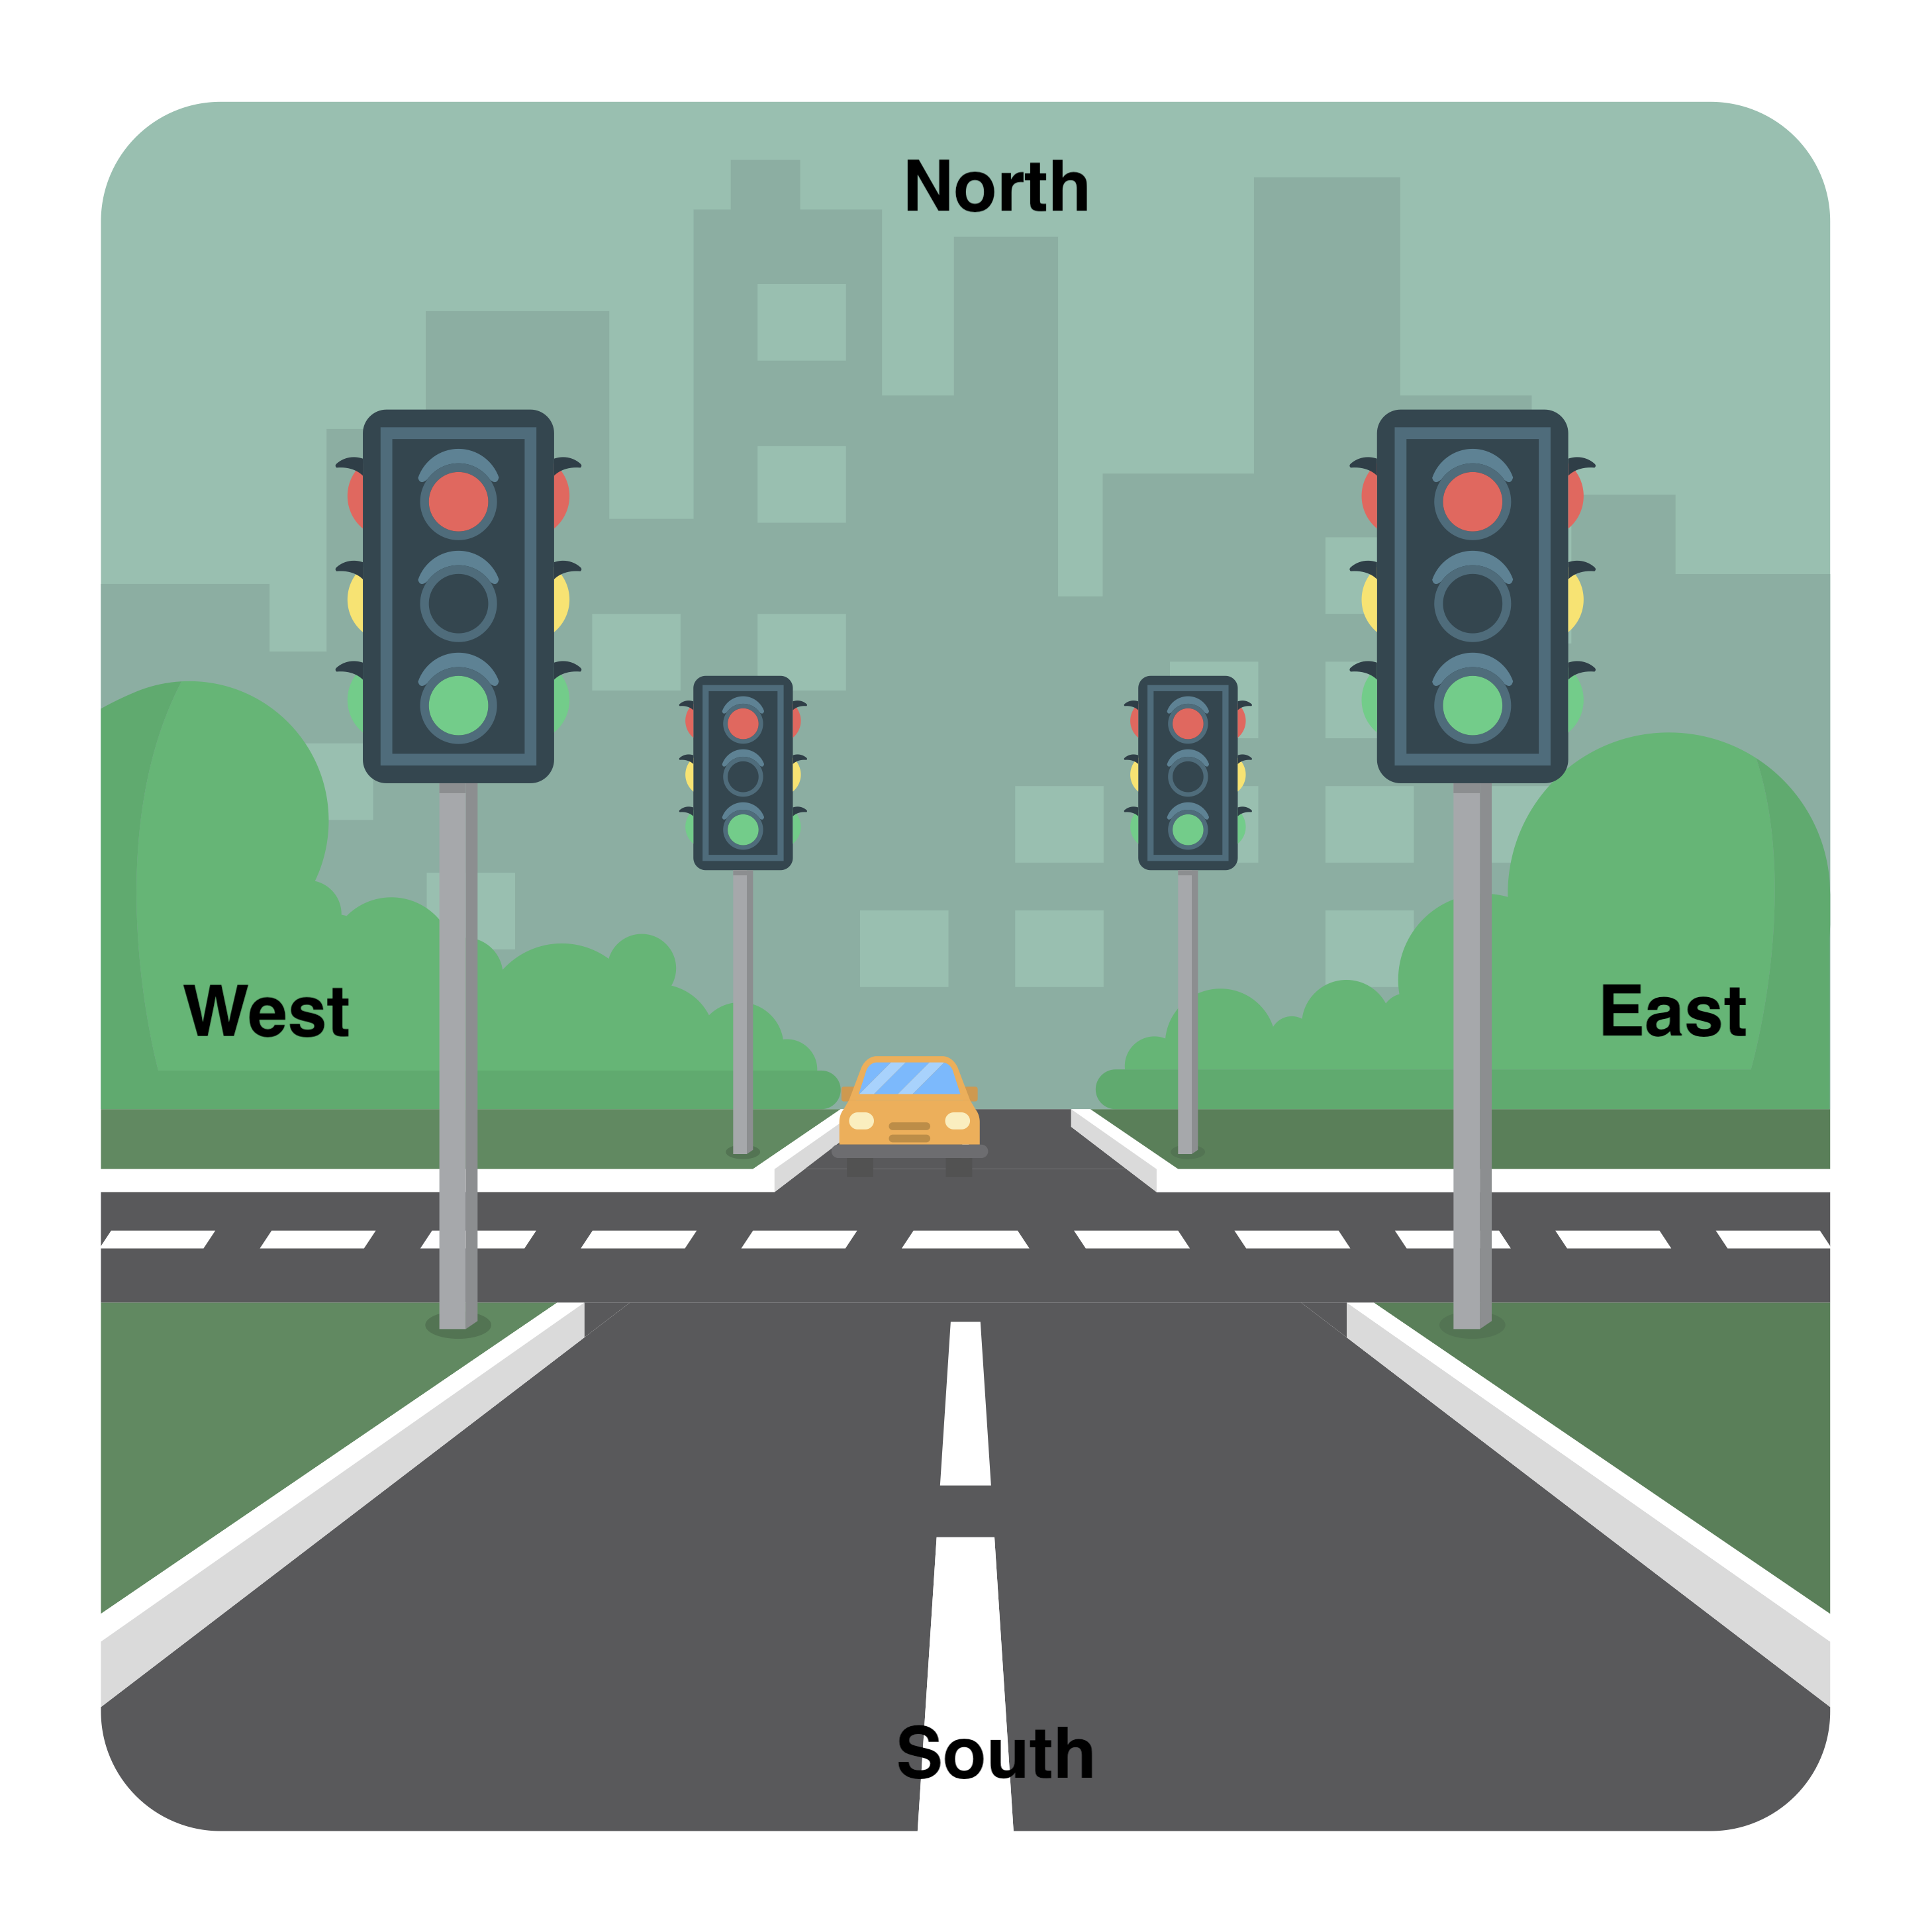
\includegraphics[width=3in]{Intersection}
\caption{Made available by Vecteezy.com}
\label{fig:Intersection}
\end{figure}


\begin{figure*}[t]
\centering
\textbf{The Final Problem - State Machine Diagram}\par
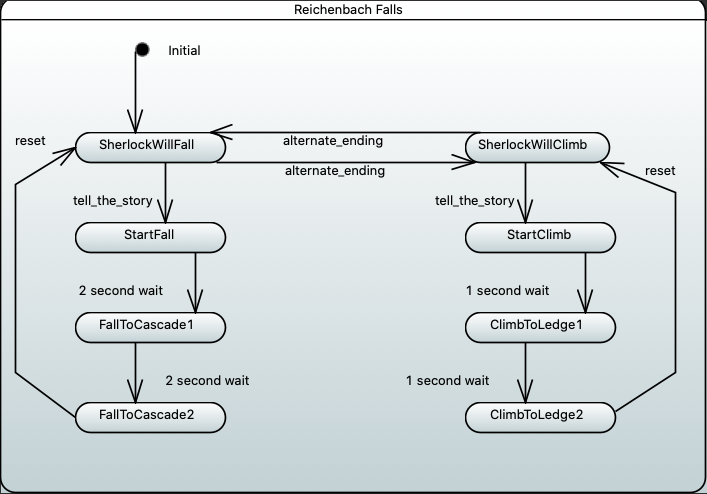
\includegraphics[width=6in, height=3in]{ReichenbachFallsStateDiagram}
\caption{State machine diagram for the final problem}
\label{fig:FinalProblemStateMachine}
\end{figure*}

\aside{The first 3 light traffic signal was invented in 1920 by William Potts, a police officer in Detroit. The older style of stoplight only had two lights and did not give drivers any warning before changing from green to red. This creates an obvious stopping problem if the driver is going at a high speed. By adding the amber light Potts resolved this issue.}

\subsection{Hint}

Each of the 12 lights should be outputs controlled by the current state. The sensors in the road will be the inputs. These sensors will have to be simulated on the HMI with push buttons. Don't forget that the sensor has to be on for an entire second before the car is considered to be waiting. The outputs should be shown on the HMI as multi-state indicators. 

Some state transitions will be based on timers...

\TASignatureSlot



\section{Challenge - The Final Problem}
Notice that there is no associated object for this lab. You must create all the necessary tags and HMI objects to fulfill the requirements outlined in this exercise. Make sure that the HMI page you make looks \textit{very} professional. 

This lab deals with state machines. In general you will need to fully define any state machine which you intend to program. However, in this part of the lab you are given the plain English description and the state machine diagram. You will have to supply everything else.

\subsection{Plain English Description}

The challenge organization has decided that this week will be the last challenge. They call it the Reichenbach machine. Reichenbach refers to the Reichenbach Falls in Switzerland. These falls were made famous in Sir Arthur Conan Doyle's Sherlock Holmes stories as the site of Holmes' alleged death.

The challenge is to have a depiction of the waterfall on the HMI. The depiction will need to include two cascades below Holmes' starting point and two ledges above. There is to be a button on the HMI which is labeled "tell the story". When the button is pressed, you are to depict Sherlock descending the 2 cascades to his doom. He should be on each of the cascades for 2 seconds.

However, there is to be another button labeled "alternate ending". This button will toggle the function of the "tell the story" button. After pressing the "alternate ending" button, the "tell the story" button should instead depict Sherlock climbing the two ledges above to secretly reach safety. When Sherlock climbs to safety, he spends 1 second on each of the two ledges. Finally there is to be a button labeled "reset" that will bring Sherlock back to the top of the falls.

Refer to \figureautorefname \ref{fig:FinalProblemStateMachine} for any additional information.

\subsection{How to make Sherlock move}

To be able to show Sherlock on the ledges and the cascades you will need to put a representation of him on the HMI. You may do this however, you see fit. However, you choose to represent Sherlock you will need to show him descending the cascades and ascending the ledges. 

It would be difficult to actually show him move (like the ball in the maze problem). Instead, it is easier to have multiple copies of your Sherlock representation on the screen at the various required locations. You can then control which of these Sherlocks is visible at a given moment. 

To control if something is visible programmatically, right click the object whose visibility you wish to control and select animation. In the animation dropdown, select visibility. In the menu that appears you can associate the objects visibility with the value stored in a particular tag in the PLC. If the tag contains the value \verb|True|, then the object is visible. Otherwise, it will not be visible on the HMI.

\TASignatureSlot